\begin{figure}[t]
\centering
\begin{subfigure}[t]{0.32\textwidth}
  \centering
  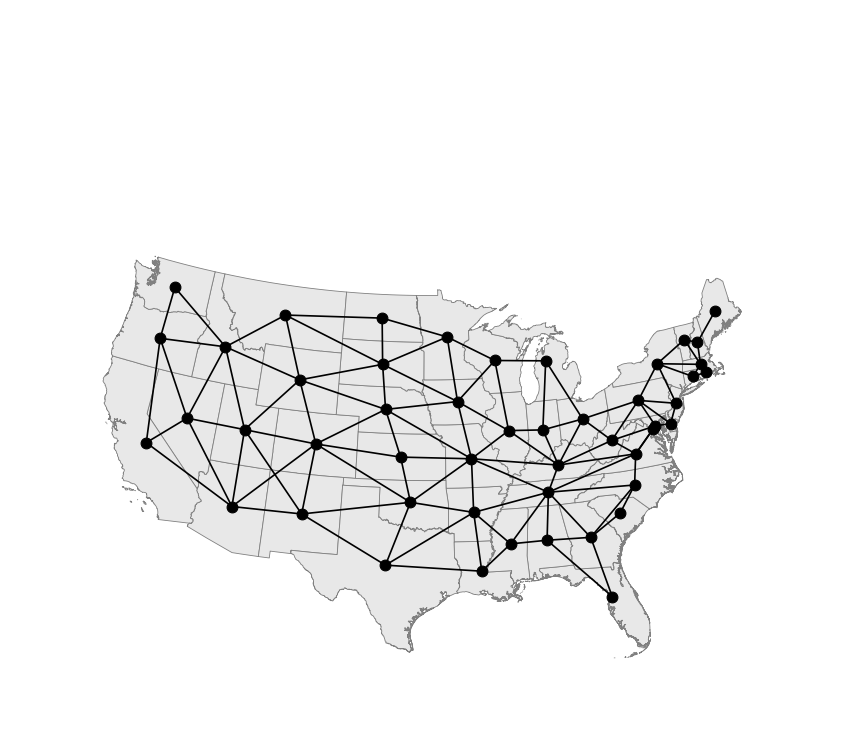
\includegraphics[width=\textwidth]{figures/dual_graph_a}
  \caption{Geographic units with dual graph $G$.}
  \label{fig:dual:a}
\end{subfigure}
\hfill
\begin{subfigure}[t]{0.32\textwidth}
  \centering
  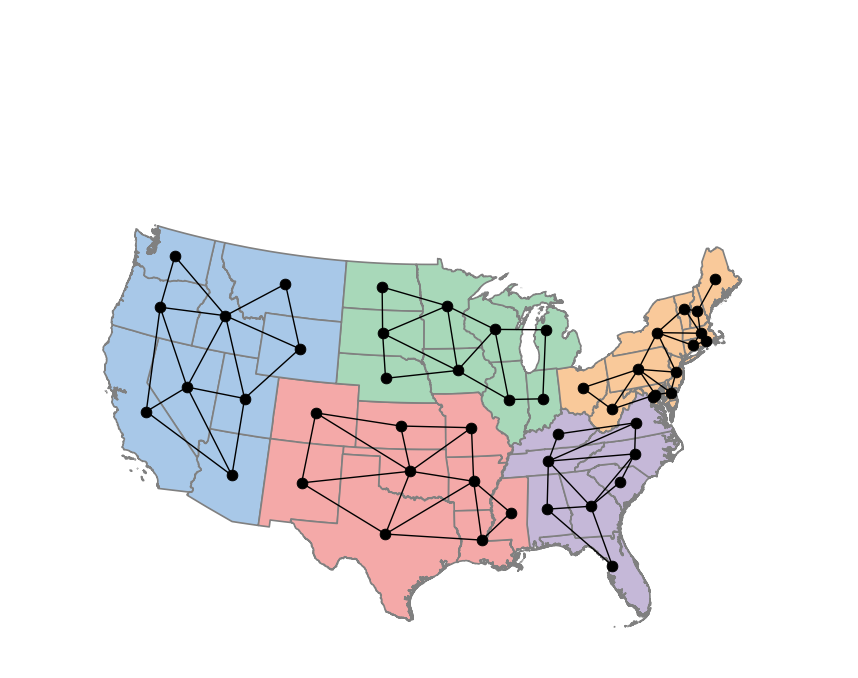
\includegraphics[width=\textwidth]{figures/dual_graph_b}
  \caption{A partition of $G^1$ into $k=6$ contiguous districts.}
  \label{fig:dual:b}
\end{subfigure}
\hfill
\begin{subfigure}[t]{0.32\textwidth}
  \centering
  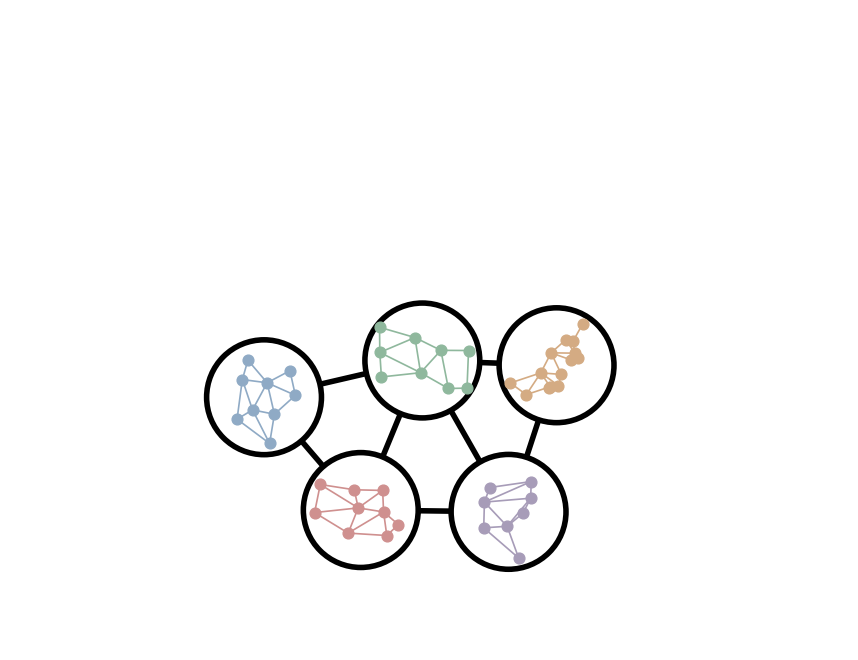
\includegraphics[width=\textwidth]{figures/dual_graph_c}
  \caption{Supergraph $G^{2}$. Each supernode represents a district.}
  \label{fig:dual:c}
\end{subfigure}
\caption{From geographic units to the supergraph used by FalCom.}
\label{fig:dual}
\end{figure}
